Unfortunately we weren't able to get a MOT which lasted longer than a few seconds. This was due to the error signal for locking the cooling laser. The error signal had a frequency bias such that the desired frequency lied outside the linear part. Therefore there was no efficient feedback and the laser could easily jump to another frequency and we were effectively working with a non locked laser. We wanted to adjust the error signal, but this was denied by the tutor.

So in all following measurements we weren't able to do a full series of measurements with one MOT but rather created a new MOT every time. Errors will be calculated by Gaussian error propagation.

\subsection{Measured data}

Lense diameter: $\si{(38 \pm 3)\, \milli\meter}$

Distance between lense and MOT: $\si{(260 \pm 10)\,\milli\meter}$

Cooling beam power: $\si{(1.2 \pm 0.1)\,mW}$ per axis

Total beam power: $\si{(3.15 \pm 0.01)\,mW}$ per axis

\subsection{Beam size}

\begin{figure}
\centering
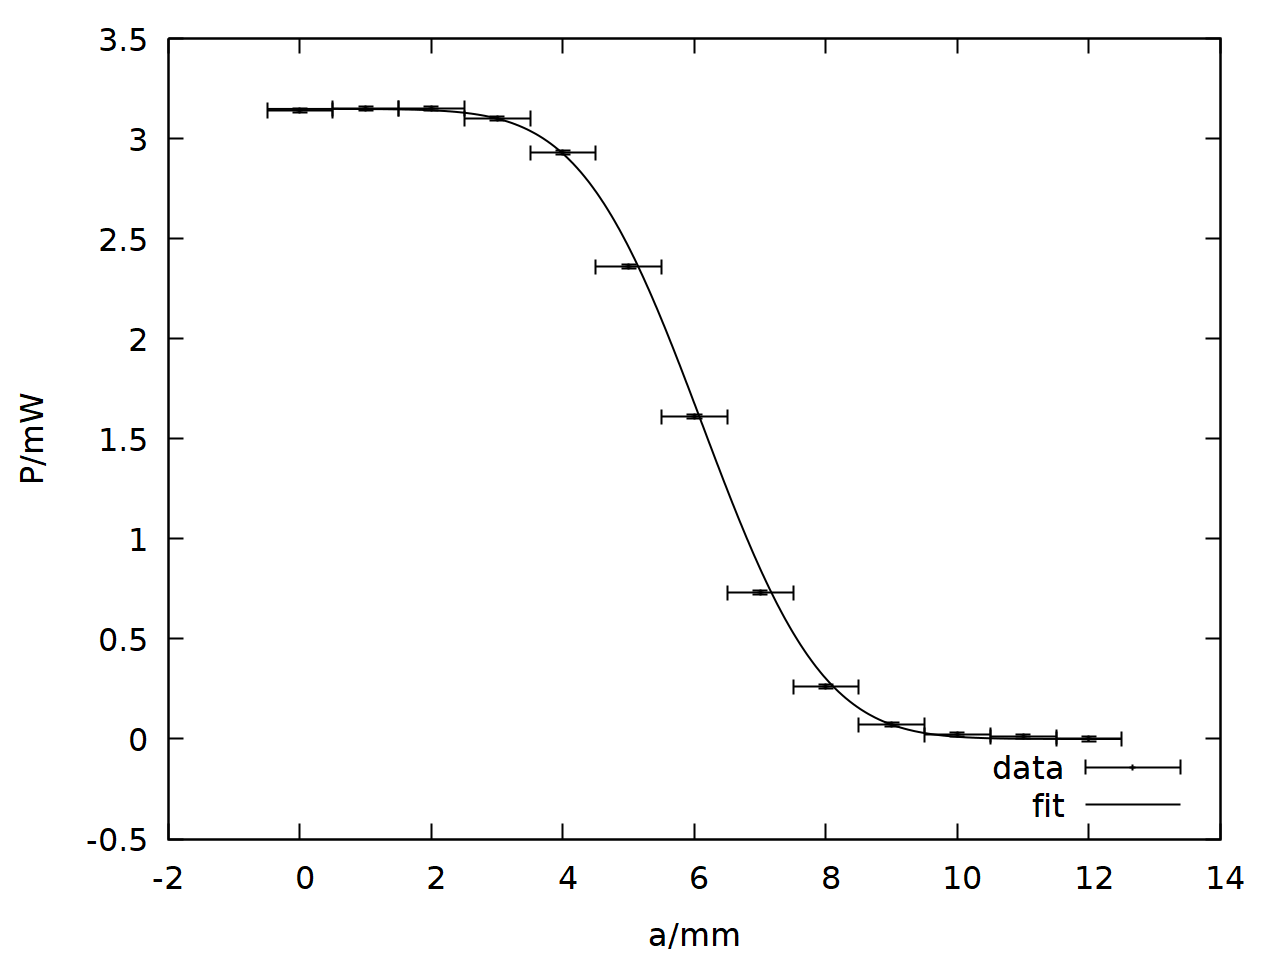
\includegraphics[width=0.7\textwidth]{data/beam.png}
\caption{Beam power over razor blade position and fit}
\label{fig:beam}
\end{figure}

The beam power is plotted over the position $a$ of the razor blade in figure \ref{fig:beam}. Since we assume a Gaussian beam the power is given by the error function, precisely $P(a) = A\qty(1-\erf(\frac{a-B}{\sqrt{2}\sigma}))$. Fitting this function to the data results in $A = \si{(1.574 \pm 0.002) mW}, B = \si{(6.12 \pm 0.09) mm}, \sigma = \si{(1.45 \pm 0.06) mm}$. The $1/e^2$ radius is then given by $4 \sigma = \si{(5.8 \pm 0.2) mm}$.

\subsection{Size of MOT}
In figure \ref{fig:mot} the MOT has dimensions $58\si{px} \times 23\si{px}$. 

\begin{figure}
\centering
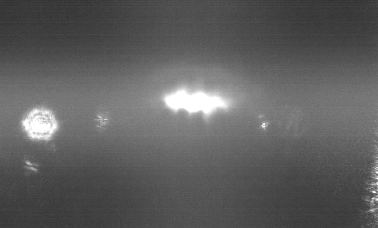
\includegraphics[width=0.7\textwidth]{figures/P102018/mot_2.png}
\caption{Picture of the MOT}
\label{fig:mot}
\end{figure}

Figure \ref{fig:karton} was taken with the same camera settings. The "Bayer Makrolon" measures $\si{(21.5 \pm 0.5) \milli\meter}$ in reality and $575 \si{px}$on the foto.

\begin{figure}
\centering
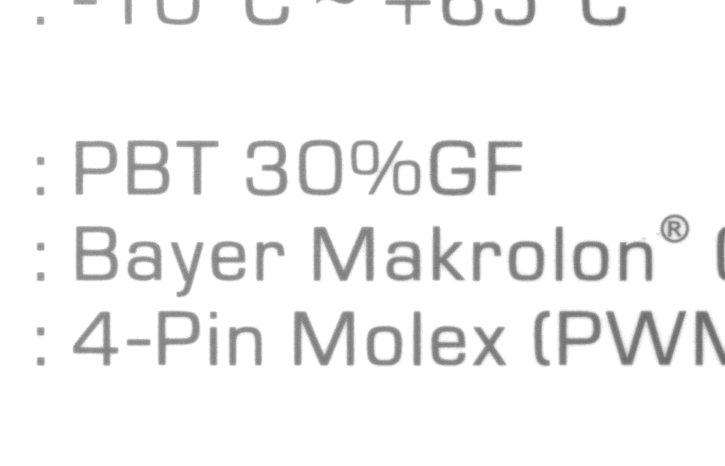
\includegraphics[width=0.7\textwidth]{figures/P102018/karton.png}
\caption{Picture of some text}
\label{fig:karton}
\end{figure}

Using this gauge one can compute the dimensions of the MOT: $\si{(2.2 \pm 0.5) \milli\meter \times (0.86 \pm 0.02) \milli\meter}$. Unfortunately we don't have information about the size of the MOT in z-direction.

\subsection{Influence of the quarter waveplate}

\begin{figure}
\centering
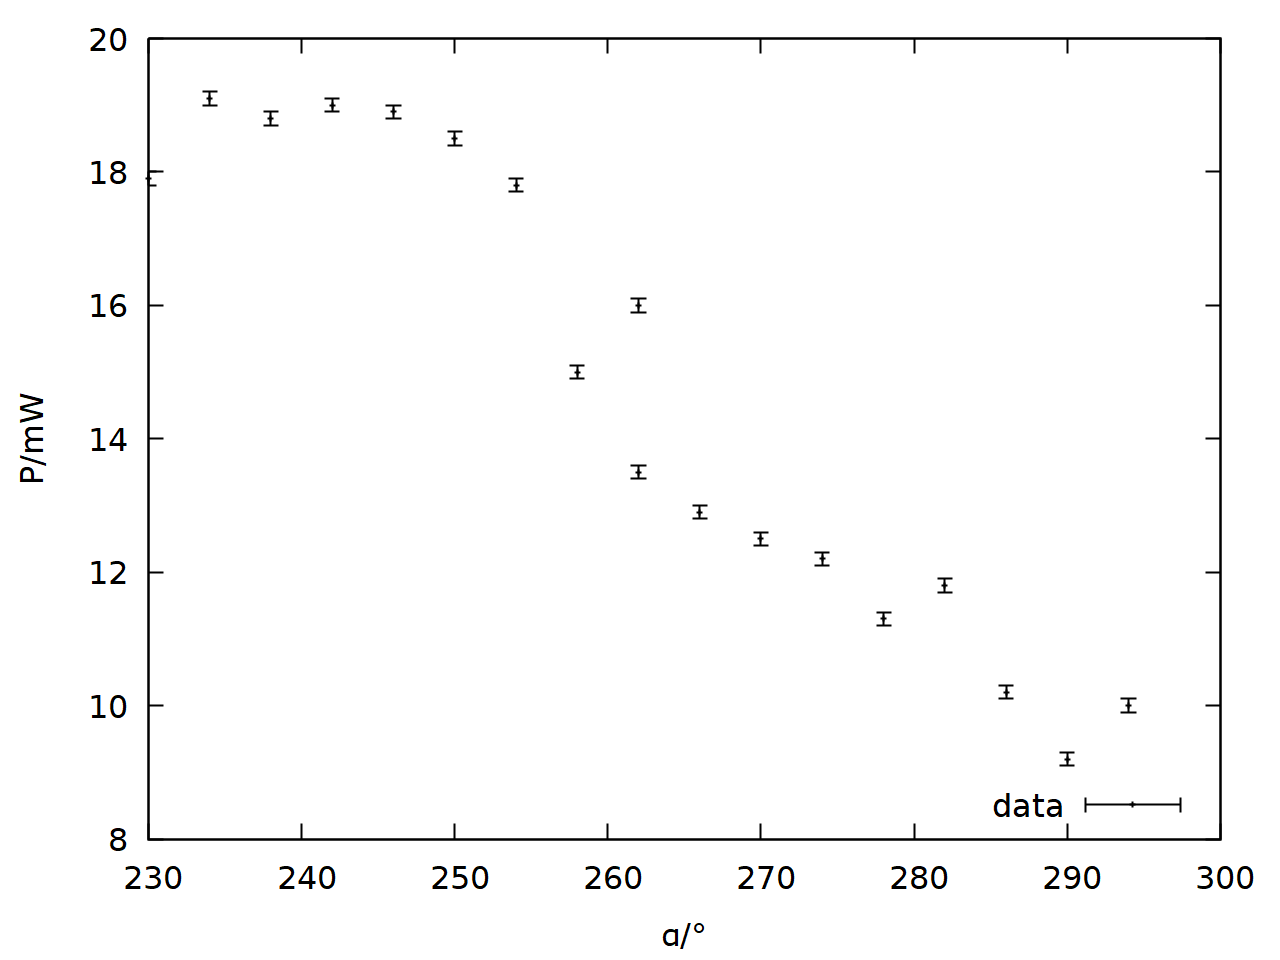
\includegraphics[width=0.7\textwidth]{data/l42.png}
\caption{Influence of the first quarter waveplate}
\label{fig:l42}
\end{figure}

\begin{figure}
\centering
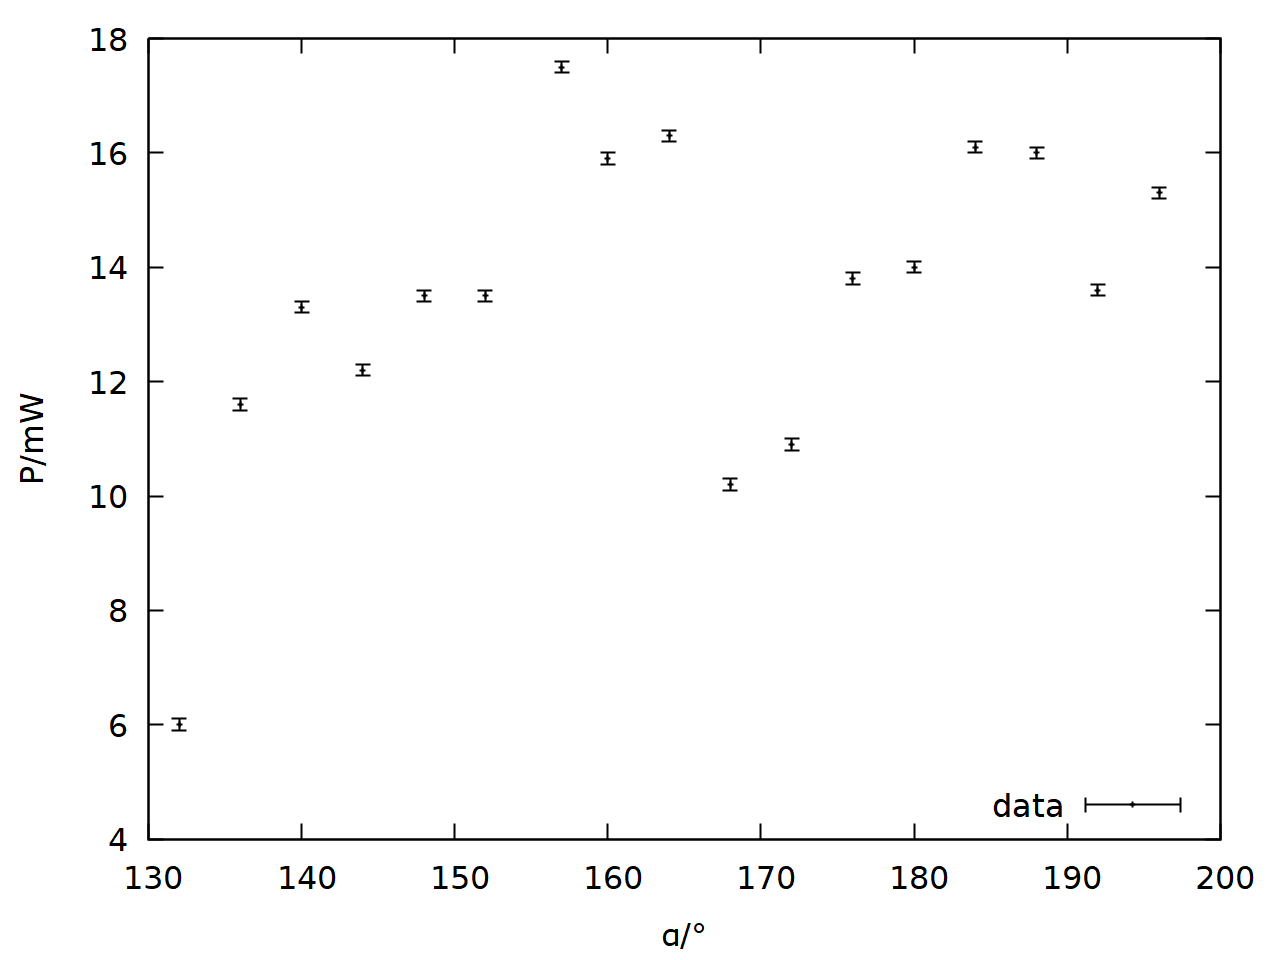
\includegraphics[width=0.7\textwidth]{data/l41.png}
\caption{Influence of the second quarter waveplate}
\label{fig:l41}
\end{figure}

In figures \ref{fig:l42} and \ref{fig:l41} the influence of the quarter waveplates on the power is given. The first waveplate (incoming beam) shows a clear drop of the power as the angle increases. As one rotates the quarter waveplate the outcoming light becomes more and more elliptical polarised. Since only the circular polarised part creates a force on the atoms this force becomes weaker and therefore less atoms will be stored in the trap. So the intensity goes down.

The second waveplate (reflected beam) shows no sensible dependence on the angle. In theory there should not be any difference, since circular polarised light has no preferred angle and therefore all angles will yield the same result. However note that we had to create a new MOT for every measurement. We think that this the causes the variation of the power for different angles.

\subsection{Changing the magnetic field}

\begin{figure}
\centering
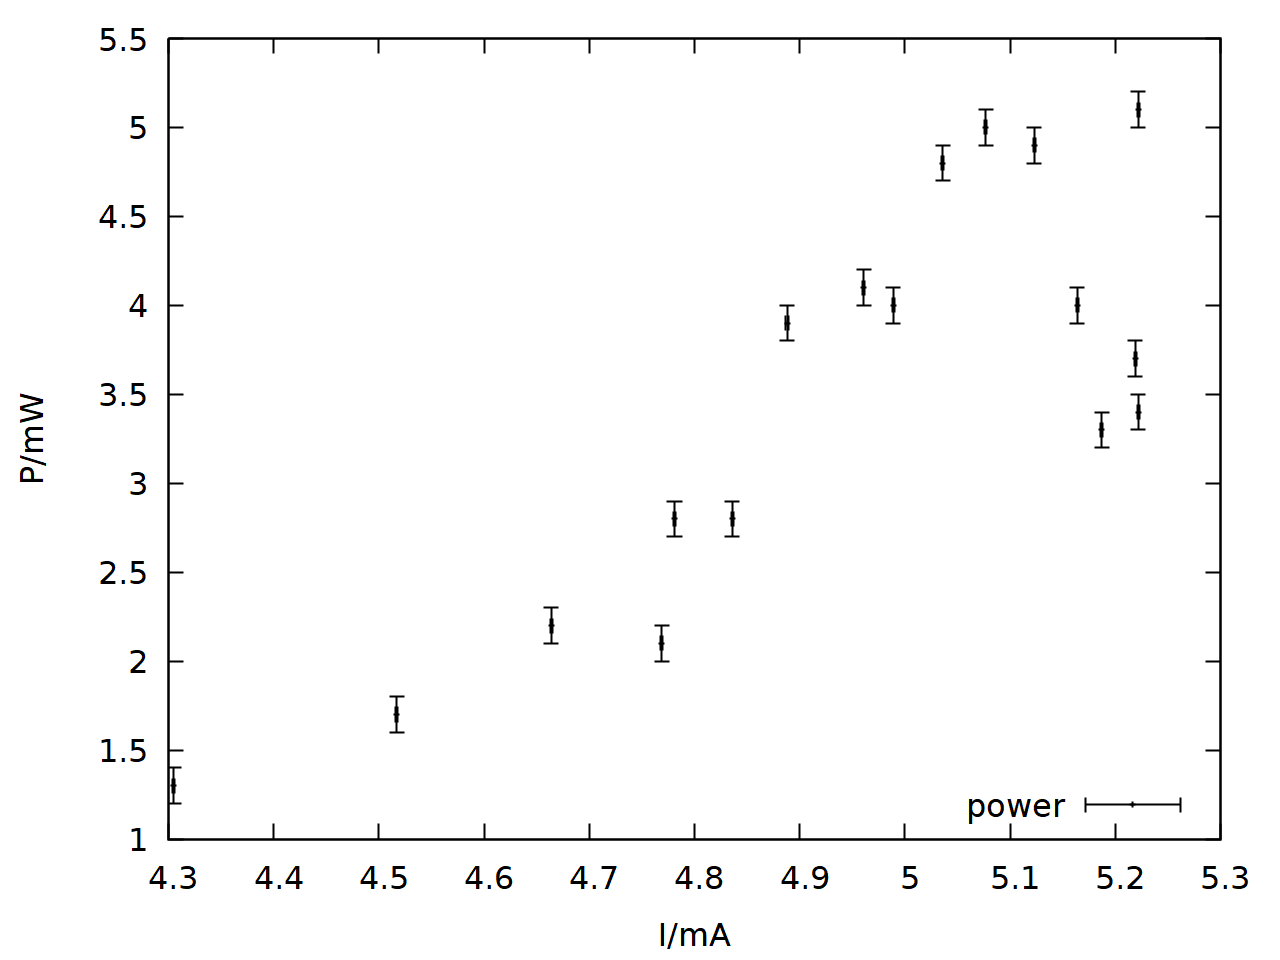
\includegraphics[width=0.7\textwidth]{data/bfeld.png}
\caption{Observed power over the coil current}
\label{fig:bfeld}
\end{figure}

In figure \ref{fig:bfeld} the dependence of the fluorescence on the coil current is plotted. As expected lower magnetic field results in less power. However there is a variation of the powers the maximum current. Again we expect this is due to the fact that we needed to create a new MOT every time. The three rightmost data points were all take at the same current and their observed powers deviate a lot. Therefore redoing the MOT every time results in a significant error.  

\subsection{Loading behaviour}
Unfortunately we weren't able to observe the loading behaviour. The tutor told us we should rather measure the detuning of the laser frequency. The pump controller had a current of $0.4 \si{\milli\ampere}$ which corresponds to approximately $0.14 \cdot 10^{-3} \si{\pascal}$.

\subsection{Detuning of the laser frequency}

\begin{figure}
\centering
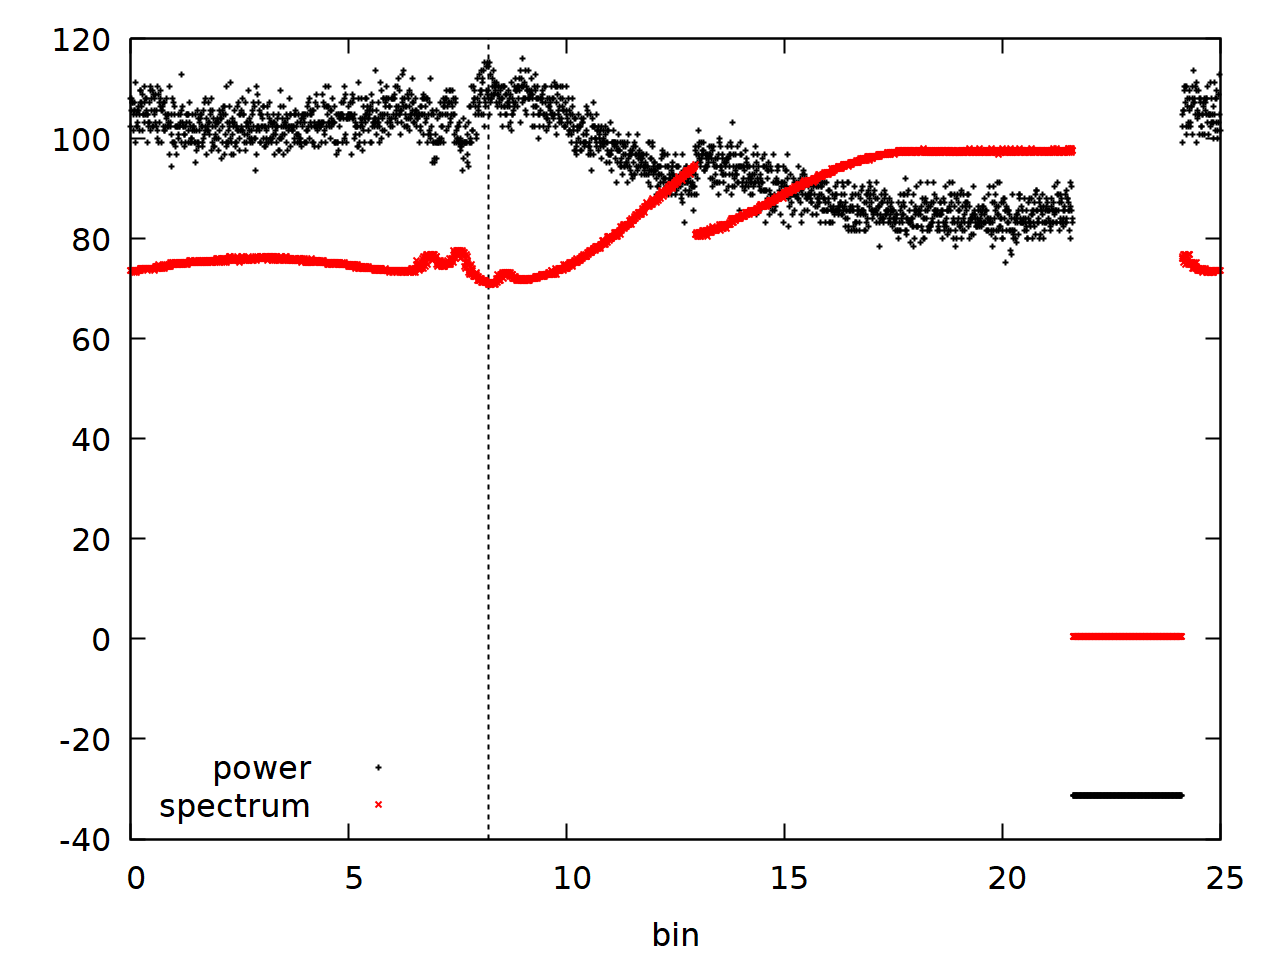
\includegraphics[width=0.7\textwidth]{data/oszi.png}
\caption{Observed power and according frequency spectrum (y-axis in arbitrary units). The dotted line represents the position of the MOT.}
\label{fig:oszi}
\end{figure}

In figure \ref{fig:oszi} the observed power as function of the frequency (in bins) is given.

The position of the maximum of power is at $(8.2 \pm 0.1) \mathrm{bin}$. The leftmost peak is at $(6.9 \pm 0.1) \mathrm{bin}$ and the rightmost at $(8.6 \pm 0.1) \mathrm{bin}$. The difference between the two peaks is then $(0.7 \pm 0.1) \mathrm{bin}$ which equals (according to our lab instructions \cite{material_tutor}) $92 \si{\mega \hertz}$. Using this one can calculate the detuning to $(0.4 \pm 0.1) \mathrm{bin} = (37 \pm 9)\si{\mega \hertz}$. 

